\documentclass[11pt]{article}
\usepackage{icmlko}
\begin{document}

\title{벽이 물러졌다 --- 깊이가 벌어 준 것으로 전이를 산다}
\author{월드모델 실험실}
\date{노트 407 · 2026년 8월 1일}
\maketitle

\begin{abstract}
노트 399가 맞바꿈을 값으로 매겼다 --- 도메인 원핫을 빼면 판 $0.0117$ 을
내고 안 본 도메인의 전이를 $+0.2058$ 산다. 노트 400이 드롭아웃으로
피하려다 실패하며 \textbf{벽}이라 적었다. 그런데 그 값은 전부
\textbf{깊이 4 에서} 잰 것이었고, 노트 405가 \textbf{깊이가 원핫을
대신한다}는 것을 보였다. 사전 등록했다 --- \emph{깊이 6 에서는 같은
맞바꿈이 더 싸야 한다.}

\begin{center}
\begin{tabular}{lrr}
\hline
 & 판(씨앗 12평균) & KR 만화 전이 \\
\hline
깊이4 · 원핫O \emph{(옛 챔피언)} & $0.4477$ & $-0.1261$ \\
깊이4 · 원핫X & $0.4359$ & $+0.0797$ \\
깊이6 · 원핫O \emph{(현 챔피언)} & $\mathbf{0.4659}$ & $-0.0822$ \\
\textbf{깊이6 · 원핫X} & $0.4616$ & $\mathbf{+0.0885}$ \\
\hline
\end{tabular}
\end{center}

\textbf{값이 반으로 떨어졌다} --- 원핫 제거가 판에 물리는 값이 짝 12뽑기로
$0.0117 \to \mathbf{0.0052}$ 다(둘 다 $0/12$). 그리고 더 중요한 것:
\textbf{깊이6·원핫X 가 깊이4 의 두 점을 \emph{둘 다} 이긴다} --- 판도 높고
($0.4616 > 0.4477$, $> 0.4359$) 전이도 높다($+0.0885 > +0.0797$,
$\gg -0.1261$). \textbf{옛 챔피언보다 판이 높으면서 전이가 양수인 모형이
처음 나왔다.}
\end{abstract}

\section{규약은 여전히 지키라 한다}

현 챔피언과 견주면 원핫 제거는 아직 $-0.0052 \cdot 0/12$ 다. 노트 378
조건 ① --- 부호가 $0/12 \le 3/12$ --- 이 걸리므로 \textbf{판이 정하고,
판은 유지라 한다. 안 바꿨다.}

노트 399가 적은 긴장이 그대로다: \emph{판은 지키라 하고 목표는 빼라 한다.}
달라진 것은 \textbf{긴장의 크기}다. 전이 한 단위를 사는 값이
$0.0117/0.2058 = 5.7\%$ 에서 $0.0052/0.1707 = \mathbf{3.0\%}$ 로 절반이
됐다. 벽은 아직 있지만 \textbf{벽의 높이는 손잡이 하나로 반이 됐고, 그
손잡이는 2년째 죽은 것으로 되어 있었다}(노트 406).

\section{누가 원핫을 아쉬워하나}

깊이 6 에서 원핫을 빼면 도서가 $+0.0213$ 으로 제일 많이 벌고 팝업이
$+0.0142$ 로 뒤따른다. 잃는 쪽은 아이돌 $-0.0784$ · 게임 $-0.0288$ ·
시장팝업 $-0.0221$ 이다.

\textbf{도서는 노트 404가 표시자 무늬 순도 $0.000$ 을 매긴 바로 그
도메인}이다 --- 축 구성이 만화와 겹쳐 무늬만으로는 제 이름을 못 부른다.
제 원핫이 정보를 못 실어 나르는 도메인이 제거로 제일 많이 번다. 노트 404의
셈이 부호를 맞혔다. 다만 $n{=}11$ 이고 노트 401이 같은 자리에서 한 번
속았으므로 \textbf{법칙이라 적지 않는다.}

\section{남은 것}

\begin{tabular}{lp{7.2cm}}
\hline
알파와 $\tau$ & 노트 406의 규약 --- 죽은 손잡이는 자료가 자라면 다시 잰다.
깊이가 벽을 반으로 깎았으니 남은 둘도 깎을지 모른다 \\
전이 점이 둘뿐 & KR 만화와 비게임 앱. CN 만화는 2025+ 가 19행이라 못 쟀다.
\textbf{$+0.0885 \pm$ 얼마인지}를 아직 모른다 \\
셋째 축 & 판과 전이를 한 축에 놓는 판정 규약이 없다. 지금은 사람이
``안 바꿨다''를 쓴다 \\
\hline
\end{tabular}

\begin{figure}[h]
\centering
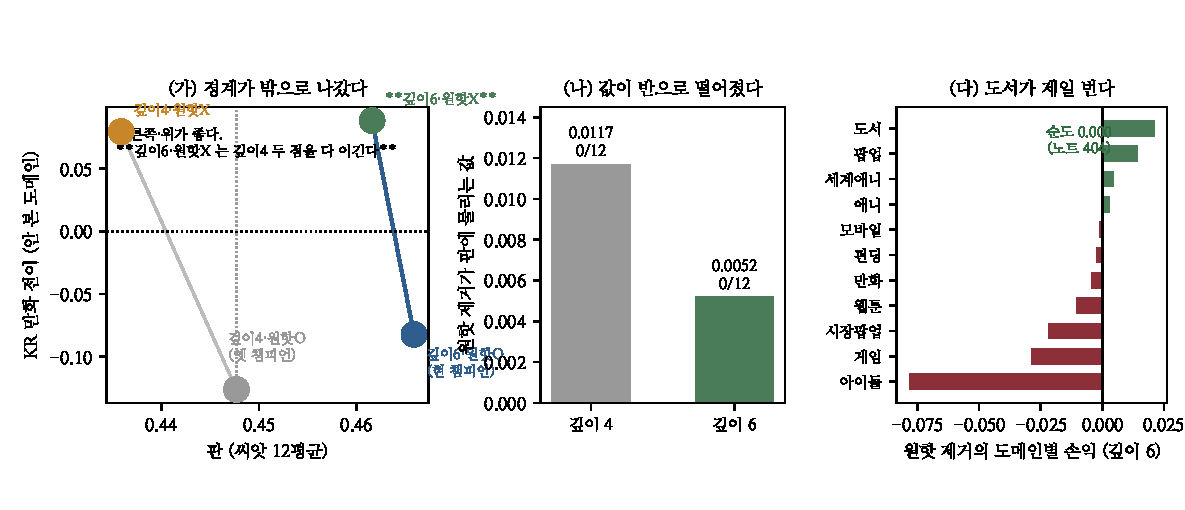
\includegraphics[width=\textwidth]{figs/fig407.pdf}
\caption{(가) 네 구성. 오른쪽·위가 좋다 --- 깊이6·원핫X 가 깊이4 의 두 점을
둘 다 이긴다. (나) 원핫 제거가 판에 물리는 값이 반으로. (다) 깊이 6 에서
원핫 제거의 도메인별 손익 --- 순도 $0.000$ 인 도서가 제일 번다.}
\end{figure}

\end{document}
